\section{RESULT AND DISCUSSION}
\hspace{1.27cm}
The first step of our simulation is initialization. The robot model, sensors model, and simulated room are loaded into the Gazebo simulator. For the sensor's data, it is also taking into account for the noise and the uncertainty in the simulation. For the second step, we create an occupancy grid map to represent the simulated room. To do that, we use the SLAM algorithm. After the model is loaded into the simulator, we run the SLAM algorithm on the background and drive the robot manually to explore the room until SLAM create a full map. We drive the robot using keyboard input and publish its data on ("/cmd\_vel") for ROS. The result of the map obtained from SLAM is shown in \textbf{Section 7.1}. For the third step, after the map is obtained, the A* is used for finding the path from start to goal in the map. On ROS the path is published on ("/path"). The result of the path from A* is shown in \textbf{Section 7.2}. Finally, the robot controller is used to control the robot while EKF is localizing the robot pose in the map. The result of control path is shown in \textbf{Section 7.3}. \textbf{\tableautorefname{ \ref{Table: Simulation Parameters}}} and \textbf{\tableautorefname{ \ref{Table: Sensor and Algorithm Data Publication Rate for EKF}}} show the initialize parameter and the rate of data publishing.\par


%First, the robot model and the sensor model is loaded in to the Gazebo simulator. And two room models is loaded: "Map1" and "Map2". Second, the robot is driven around the room by keyboard command ("/cmd\_vel") while the SLAM algorithm is running to create the occupancy grid map ("/map"). Third, the A* is used to search the path from start to goal in the map ("/path"). Finally, the robot controller is used to control the robot while EKF is localizing the robot pose in the map. \textbf{\tableautorefname{ \ref{Table: Simulation Parameters}}} and \textbf{\tableautorefname{ \ref{Table: Sensor and Algorithm Data Publication Rate for EKF}}} show the initialize parameter and the rate of data publishing.\par


\begin{table}[ht]
	\begin{center}
		\caption{Simulation Parameters}
		\label{Table: Simulation Parameters}
		\begin{tabular}{ccc}
			Parameter                    &Value                              &Unit           \\
			\hline
			k1                           &5                                  &-              \\
			k2                           &10                                 &-              \\
			k3                           &10                                 &-              \\
			ka                           &15                                 &-              \\
			kb                           &15                                 &-              \\
			$r$                          &0.1                                &$m$            \\
			$L$                          &0.2                                &$m$            \\
			Q                            &$diag(1^2,0.52^2)\times 0.01$      &-              \\
			R                            &$diag(1^2,1^2,1^2)\times 0.01$     &-              \\
			%\hline
			\ChangeRT{1.5pt} 
		\end{tabular}
	\end{center}
\end{table}


\begin{table}[ht]
	\begin{center}
		\caption{Sensor and Algorithm Data Publication Rate for EKF}
		\label{Table: Sensor and Algorithm Data Publication Rate for EKF}
		\begin{tabular}{ccc}
			Data Publish                 &Rate             &Unit            \\
			\hline
			Encoder                      &20               &Hz              \\
			IMU                          &10               &Hz              \\
			Lidar Scan Match             &30               &Hz              \\
			EKF Fusion                   &20               &Hz              \\
			%\hline
			\ChangeRT{1.5pt} 
		\end{tabular}
	\end{center}
\end{table}



\textbf{\figureautorefname{ \ref{fig:Robot Model Simulation}}} shows the Differential Drive Wheeled Mobile Robot and Sensors (IMU, Lidar, Wheel Encoder) 3D model that is viewed inside Gazebo Simulator. \textbf{\figureautorefname{ \ref{fig:Map1 and Map2 in simulation}}} shows the 3D models of simulated rooms.

% Figure Image =============================================================================
\begin{figure}[ht]
	\centering
	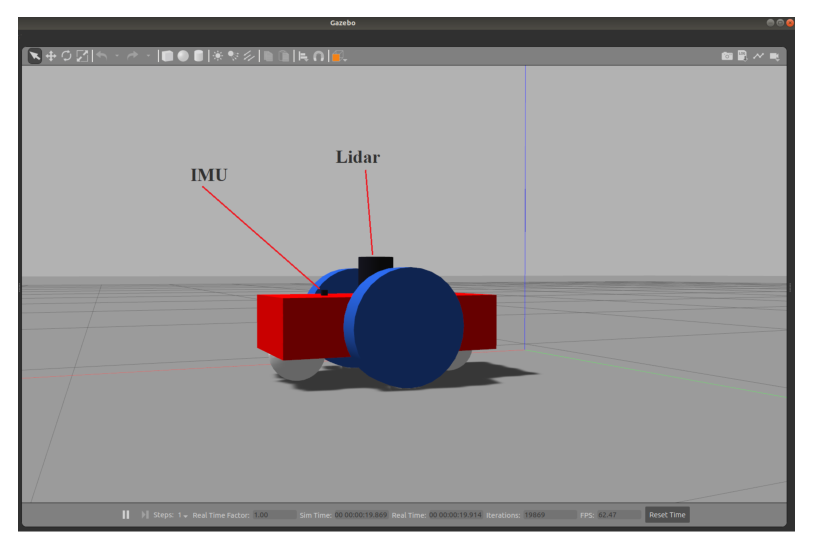
\includegraphics[scale=1]{images/imagess/3method-gazebo.eps} 
	\caption{Robot Model Simulation}
	\label{fig:Robot Model Simulation}
\end{figure}
% Figure Image =============================================================================

\begin{figure}[H]
	\centering
	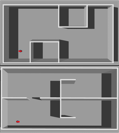
\includegraphics[scale=1]{images/imagess/7reslt-map1and2.pdf} 
	\caption{Map1 and Map2 in simulation}
	\label{fig:Map1 and Map2 in simulation}
\end{figure}



\subsection{SLAM}
% SLAM
\hspace{1.27cm}
In this section, we show the result from the SLAM algorithm of "Map1" and "Map2". First, the robot is placed in the room at the start location. Our goal is drive the robot manually to create the map. While the SLAM algorithm is running, we use keyboard input to move the robot along the green line from start to goal location. SLAM output the occupancy grid map and is visualized using RVIZ as shown in \textbf{\figureautorefname{ \ref{fig:Map1 SLAM}}} and \textbf{\figureautorefname{ \ref{fig:Map2 SLAM}}}. From the figures, the white space is the free space that allow the robot to move in while the black line is the obstacle.\par
\begin{figure}[H]
	\centering
	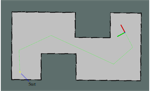
\includegraphics[scale=0.80]{images/imagess/7reslt-slam-map1.pdf}
	\caption{Map1 SLAM}
	\label{fig:Map1 SLAM}
\end{figure}

\begin{figure}[H]
	\centering
	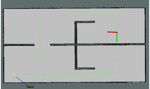
\includegraphics[scale=0.80]{images/imagess/7reslt-slam-map2.pdf}
	\caption{Map2 SLAM}
	\label{fig:Map2 SLAM}
\end{figure}
Hector SLAM algorithm build an accurate occupancy grid map from the simulated room.



\subsection{Path Planning}
\hspace{1.27cm}
In this section, we show the result of the A* path planning algorithm of "Map1" and "Map2". After the occupancy grid map from the previous section is build, we put the robot at a resting state on the start location on the map. Then we chose the goal location that we want the robot to go. The A* algorithm calculates an optimal path from the map and those 2 locations and output a trajectory of the robot to follow in brown line as in \textbf{\figureautorefname{ \ref{fig:Map1 Path Planning}}} and \textbf{\figureautorefname{ \ref{fig:Map2 Path Planning}}}. As the algorithm is in function with Heuristic function, the H value should not be overestimated.\par


%In this section, the path is searched from start to goal point using the A*. The start point is chosen to be the current pose of the robot and the goal point is where we put in the location that we want the robot to go. In the figure below, the brown line is the path that the algorithm generated.

\begin{figure}[H]
	\centering
	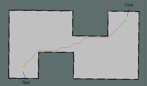
\includegraphics[scale=0.80]{images/imagess/7reslt-pp-map1.pdf}
	\caption{Map1 Path Planning}
	\label{fig:Map1 Path Planning}
\end{figure}

\begin{figure}[H]
	\centering
	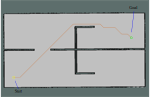
\includegraphics[scale=0.80]{images/imagess/7reslt-pp-map2.pdf}
	\caption{Map2 Path Planning}
	\label{fig:Map2 Path Planning}
\end{figure}




\subsection{Control}
\hspace{1.27cm}
In this section, we show the control of the robot path from start to goal. After the trajectory is generated from the A* from the last section, the controller is required to move the robot. The backstepping controller calculate the required linear velocity and angular velocity from the trajectory and the current position of the robot. To keep track of robot position, the EKF is used to estimated it location and feedback to the controller. For better performance, the constants variable in \textbf{\tableautorefname{ \ref{Table: Simulation Parameters}}} is manually tuned. In the \textbf{\figureautorefname{ \ref{fig:Map1 Control}}} and \textbf{\figureautorefname{ \ref{fig:Map2 Control}}}, the brown line is the path that the algorithm generated. The blue line is the path that the robot currently move. As seen in the figures, the blue line follow the brown line accurately which mean the control performance is acceptable.\par


\begin{figure}[H]
	\centering
	\includegraphics[scale=0.75]{images/imagess/7reslt-cntrl-map1.pdf}
	\caption{Map1 Control}
	\label{fig:Map1 Control}
\end{figure}

\begin{figure}[H]
	\centering
	\includegraphics[scale=0.75]{images/imagess/7reslt-cntrl-map2.pdf}
	\caption{Map2 Control}
	\label{fig:Map2 Control}
\end{figure}